\documentclass[11pt,letterpaper]{article}
\usepackage[T1]{fontenc}
\usepackage[utf8]{inputenc}
\usepackage{lmodern}
\usepackage[margin=1in]{geometry}
\usepackage{amsmath,amssymb,amsthm,mathtools}
\usepackage{microtype,booktabs,graphicx,array}
\usepackage{enumitem,listings,fancyhdr,placeins}
\usepackage[hidelinks]{hyperref}
\hypersetup{pdftitle={The maximal positive coefficient of a Hermite polynomial},pdfsubject={Exact maximization and asymptotics of OEIS A277280}}
\setlength{\parindent}{0pt}
\setlength{\parskip}{0.45em}
\setlength{\headheight}{14pt}
\pagestyle{fancy}
\fancyhf{}
\fancyhead[L]{\small A277280: exact maximum and asymptotics}
\fancyhead[R]{\small\thepage}
\renewcommand{\headrulewidth}{0.3pt}
\newtheorem{theorem}{Theorem}[section]
\newtheorem{proposition}[theorem]{Proposition}
\newtheorem{lemma}[theorem]{Lemma}
\newtheorem{corollary}[theorem]{Corollary}
\theoremstyle{remark}
\newtheorem{remark}[theorem]{Remark}
\newcommand{\NN}{\mathbb{N}}
\newcommand{\ZZ}{\mathbb{Z}}
\newcommand{\RR}{\mathbb{R}}
\newcommand{\ee}{\mathrm{e}}
\newcommand{\isqrt}{\operatorname{isqrt}}
\newcommand{\dist}{\operatorname{dist}}
\newcommand{\Unif}{\operatorname{Unif}}
\newcommand{\coef}[2]{[#1]#2}
\DeclareMathOperator{\fracpart}{frac}
\lstset{language=Python,basicstyle=\small\ttfamily,columns=fullflexible,
 keepspaces=true,showstringspaces=false,breaklines=true,frame=single,
 framerule=0.3pt,xleftmargin=0.8em,xrightmargin=0.8em,aboveskip=0.9em,
 belowskip=0.9em}

\title{The maximal positive coefficient\\of a Hermite polynomial\\[0.45em]
\large Exact maximization, asymptotic growth, and lattice fluctuations}
\author{A research note on OEIS A277280}
\date{20 September 2026}

\begin{document}
\maketitle
\thispagestyle{empty}
\begin{abstract}
Let $a(n)$ be the largest coefficient of the physicists' Hermite polynomial
$H_n(x)$, with signs taken into account. We prove the full asymptotic equivalent
\[
\boxed{\displaystyle
 a(n)\sim
 \frac{\exp(\sqrt{2n}-\tfrac12)}{\sqrt{\pi}\,(2n)^{1/4}}
 \left(\frac{2n}{\ee}\right)^{n/2}.}
\]
The proof includes an exact, integer-arithmetic formula for the uniquely
maximizing exponent. A factorization reduces the apparent quartic comparison
between adjacent positive coefficients to a quadratic inequality. Uniform
Stirling expansions then give three explicit correction polynomials. The
first correction depends on a bounded rounding displacement and genuinely
oscillates; its sharp lower and upper limits and its limiting distribution
are determined. We also prove $a(n+1)/(a(n)\sqrt n)\to\sqrt2$, describe its
first-order fluctuations, and compare the answer with the maximum absolute
coefficient. Exact Python implementations, independent finite checks,
high-precision numerical tables, and reproducible figures accompany the note.
\end{abstract}

\vfill
\small
\textbf{Scope.} The sequence definition and normalization are taken from
OEIS and NIST DLMF. The exact maximization, asymptotic expansions, and
fluctuation results below are proved in the text rather than inferred from
numerical fitting. No claim of a complete literature search or historical
priority is made.
\normalsize
\newpage
\tableofcontents
\newpage

\section{The sequence and the normalization}

OEIS A277280 is the maximal coefficient of $H_n(x)$, where coefficients
retain their signs \cite{oeis280}. The entry was introduced by Vladimir
Reshetnikov in October 2016. The relevant Hermite polynomials are the
\emph{physicists'} polynomials, not the differently normalized
probabilists' polynomials. Their explicit expansion is
\begin{equation}\label{eq:hermite}
 H_n(x)=n!\sum_{j=0}^{\lfloor n/2\rfloor}
 \frac{(-1)^j 2^{n-2j}x^{n-2j}}{j!\,(n-2j)!},
\end{equation}
as in DLMF 18.5.13 \cite{dlmfhermite}. In particular,
\[
 H_5(x)=32x^5-160x^3+120x,
 \qquad a(5)=120,
\]
not $160$. Zero coefficients do not affect the maximum, since the leading
coefficient $2^n$ is positive.

A coefficient in \eqref{eq:hermite} is positive precisely when $j$ is even.
Writing $j=2k$ and $d=n-4k$ gives
\begin{equation}\label{eq:maxdef}
 a(n)=\max_{0\le k\le\lfloor n/4\rfloor}
 \frac{n!\,2^{n-4k}}{(2k)!\,(n-4k)!}
 =\max_{d\in\mathcal D_n} C_n(d),
\end{equation}
where
\begin{equation}\label{eq:lattice}
 \mathcal D_n=\{d\in\ZZ:0\le d\le n,\ d\equiv n\pmod4\},
 \qquad
 C_n(d)=\frac{n!\,2^d}{((n-d)/2)!\,d!}.
\end{equation}
The distinction between a lattice of spacing $4$ and one of spacing $2$
is the entire sign constraint. It will affect lower-order terms, but not
the leading asymptotic constant.

The first terms, indexed from $n=0$, are
\[
 1,2,4,8,16,120,720,3360,13440,48384,302400,2217600,\ldots.
\]
The closely related sequence A277281 takes the maximum \emph{absolute}
coefficient instead \cite{oeis281}; Section~\ref{sec:absolute} compares the two.

\section{An exact solution of the discrete maximization}\label{sec:exact}

The maximizing coefficient can be found without constructing a polynomial,
scanning its coefficients, or evaluating any floating-point square root.

\begin{theorem}[Exact maximizing exponent]\label{thm:exact}
For every integer $n\ge0$, set
\begin{equation}\label{eq:kexact}
 k_n=\left\lfloor
 \frac{2n+6-\lfloor\sqrt{8n+21}\rfloor}{8}
 \right\rfloor,
 \qquad d_n=n-4k_n.
\end{equation}
Then $d_n$ is the unique maximizing exponent in \eqref{eq:maxdef}, and
\begin{equation}\label{eq:aexact}
 \boxed{\displaystyle
 a(n)=\frac{n!\,2^{d_n}}{(2k_n)!\,d_n!}.}
\end{equation}
Equivalently, if
\begin{equation}\label{eq:threshold}
 r_n=\frac{\sqrt{8n+21}-7}{2},
\end{equation}
then $d_n$ is the smallest allowed exponent strictly greater than $r_n$.
In fact, $r_n<d_n<r_n+4$.
\end{theorem}

\begin{proof}
For two consecutive allowed exponents $d,d+4$, put $m=(n-d)/2$.
Cancellation of factorials gives
\begin{equation}\label{eq:fourratio}
 \frac{C_n(d+4)}{C_n(d)}
 =\frac{16m(m-1)}{(d+1)(d+2)(d+3)(d+4)}
 =\frac{4(n-d)(n-d-2)}{(d+1)(d+2)(d+3)(d+4)}.
\end{equation}
The difference between the denominator and numerator has the useful
factorization
\begin{align}
 &(d+1)(d+2)(d+3)(d+4)-4(n-d)(n-d-2)\notag\\
 &\hspace{1em}=
 (d^2+7d+7-2n)(d^2+3d+3+2n)+3.\label{eq:factor}
\end{align}
For integer $d,n$, the first factor on the right is odd, hence nonzero.
The second factor is greater than $3$ whenever $d,d+4$ are both allowed.
Consequently the sign of \eqref{eq:factor} is exactly the sign of
$d^2+7d+7-2n$. Thus
\begin{equation}\label{eq:quadraticcriterion}
 C_n(d+4)>C_n(d)
 \quad\Longleftrightarrow\quad d^2+7d+7<2n.
\end{equation}
The quadratic on the left is strictly increasing for $d\ge0$ and crosses
$2n$ at $r_n$. The positive coefficients therefore increase strictly until
passing this threshold, and then decrease strictly. This proves uniqueness
and identifies the mode.

The endpoint $n$ exceeds $r_n$. For $n\ge4$, $r_n>0$, and for $n=0,1,2,3$
the asserted mode is checked immediately. Hence the lattice description
indeed gives an allowed exponent for every $n\ge0$. Solving it for $k_n$
gives
\begin{equation}\label{eq:kreal}
 k_n=\left\lfloor\frac{2n+7-\sqrt{8n+21}}{8}\right\rfloor.
\end{equation}
Now $8n+21\equiv5\pmod8$, so it is never a square. If
$q=\lfloor\sqrt{8n+21}\rfloor$, then
$\sqrt{8n+21}=q+\varepsilon$ with $0<\varepsilon<1$.
Replacing the numerator in \eqref{eq:kreal} by $2n+6-q$ does not change its
quotient's floor: the difference is $1-\varepsilon\in(0,1)$ and the latter
numerator is an integer. This proves \eqref{eq:kexact}. Substitution into
\eqref{eq:lattice} proves \eqref{eq:aexact}.
\end{proof}

\subsection{Localization and a useful rounding interpretation}

For $n\ge1$, write
\begin{equation}\label{eq:sdelta}
 s=s_n=\sqrt{2n},
 \qquad
 \delta_n=d_n-s_n+\frac32.
\end{equation}
The exact threshold has the expansion
\begin{equation}\label{eq:rexpansion}
 r_n=s_n-\frac72+\frac{21}{8s_n}+O(s_n^{-3}).
\end{equation}
It follows that
\begin{equation}\label{eq:deltabound}
 -2+\frac{21}{8s_n}+O(s_n^{-3})
 <\delta_n<
 2+\frac{21}{8s_n}+O(s_n^{-3}).
\end{equation}
In particular, $d_n=\sqrt{2n}+O(1)$, while
\[
 k_n=\frac n4-\frac{\sqrt{2n}}4+O(1).
\]
The maximizing term is therefore far below the leading degree $n$, but
not close to a fixed degree either.

Define the exact rounding center
\begin{equation}\label{eq:roundcenter}
 h_n=r_n+2=\frac{\sqrt{8n+21}-3}{2}.
\end{equation}
The exponent $d_n$ is the member of $n+4\ZZ$ nearest to $h_n$.
There is no midpoint ambiguity, because $r_n$ is not an integer.
This statement is an exact discrete rule, not an assumption that rounding
the maximum of a smooth interpolation must always work.

\section{The leading asymptotic equivalent}\label{sec:leading}

Define, for real $n>0$,
\begin{equation}\label{eq:L}
 L(n)=\frac{\exp(s_n-\tfrac12)}{\sqrt\pi\,s_n^{1/2}}
       \left(\frac{2n}{\ee}\right)^{n/2}
 =\frac{\exp(\sqrt{2n}-\tfrac12)}{\sqrt\pi\,(2n)^{1/4}}
       \left(\frac{2n}{\ee}\right)^{n/2}.
\end{equation}

\begin{theorem}[Full asymptotic growth]\label{thm:leading}
As $n\to\infty$ through the integers,
\begin{equation}\label{eq:mainequiv}
 \boxed{\displaystyle a(n)=L(n)\bigl(1+O(n^{-1/2})\bigr).}
\end{equation}
In particular $a(n)\sim L(n)$, with exactly the constant and powers displayed
in \eqref{eq:L}.
\end{theorem}

\begin{proof}
Let $d=d_n=s+O(1)$ and $N=n/2$. Extend factorials by the gamma function.
Stirling's expansion \cite{dlmfgamma} first gives
\begin{equation}\label{eq:basegamma}
 \log\frac{\Gamma(n+1)}{\Gamma(N+1)}
 =\frac n2\log\frac{2n}{\ee}+\frac12\log2+O(n^{-1}).
\end{equation}
A second application, with the moving displacement $d/2=O(\sqrt N)$,
gives
\begin{equation}\label{eq:shiftgamma}
 \log\frac{\Gamma(N+1)}{\Gamma(N-d/2+1)}
 =\frac d2\log N-\frac{d^2}{4n}+O(s^{-1}).
\end{equation}
For completeness, this follows by expanding
$\log(N-d/2)=\log N+\log(1-d/(2N))$ in the two Stirling expressions.
The neglected terms have size
$O(d/N+d^3/N^2)=O(s^{-1})$; a fixed-shift gamma-ratio formula is not
being applied outside its range of uniformity.

Combining \eqref{eq:basegamma}, \eqref{eq:shiftgamma}, and the remaining
factor $2^d/\Gamma(d+1)$ yields
\begin{align}
 \log C_n(d)
 &=\frac n2\log\frac{2n}{\ee}+\frac12\log2
   +d\log s-\log\Gamma(d+1)-\frac{d^2}{4n}
   +O(s^{-1})\notag\\
 &=\frac n2\log\frac{2n}{\ee}
   +d\log\frac{s}{d}+d
   -\frac12\log(\pi d)-\frac{d^2}{2s^2}
   +O(s^{-1}).\label{eq:basiclog}
\end{align}
Because $d=s+O(1)$,
\[
 d\log\frac{s}{d}+d=s+O(s^{-1}),\qquad
 \log d=\log s+O(s^{-1}),\qquad
 \frac{d^2}{2s^2}=\frac12+O(s^{-1}).
\]
Therefore
\begin{equation}\label{eq:logleading}
 \log a(n)=\frac n2\log\frac{2n}{\ee}+s
 -\frac12-\frac12\log\pi-\frac12\log s+O(s^{-1})
 =\log L(n)+O(s^{-1}).
\end{equation}
Exponentiating proves the theorem.
\end{proof}

\subsection{Equivalent descriptions of the growth rate}

The logarithmic form, with all constant terms made explicit, is
\begin{align}
 \log a(n)
 &=\frac n2\log n+\frac n2(\log2-1)+\sqrt{2n}
   -\frac14\log n\notag\\
 &\quad-\frac14\log2-\frac12\log\pi-\frac12
   +O(n^{-1/2}).\label{eq:fulllog}
\end{align}
Thus
\begin{equation}\label{eq:growthlimits}
 \frac{\log a(n)}{n\log n}\longrightarrow\frac12,
 \qquad
 \frac{a(n)^{1/n}}{\sqrt n}\longrightarrow\sqrt{\frac2{\ee}}.
\end{equation}
The factor $\exp(\sqrt{2n})$ is subexponential in $n$, but it cannot be
absorbed into a multiplicative constant. Similarly, the factor $n^{-1/4}$
and the constant $2^{-1/4}/\sqrt{\pi\ee}$ are needed for a true asymptotic
equivalent rather than just logarithmic growth.

\subsection{Why the sign restriction does not halve the maximum}

The coefficient peak has a width that diverges. To see this directly,
consider $C_n(d)$ with the gamma-function extension when necessary and put
$d=s+x\sqrt s$, where $x$ stays in a fixed bounded interval. The same
calculation as \eqref{eq:basiclog} is uniform on this scale, and gives
\begin{equation}\label{eq:gaussian}
 \log\frac{C_n(s+x\sqrt s)}{L(n)}
 =-\frac{x^2}{2}+O(s^{-1/2}).
\end{equation}
Indeed, the main varying term is
\[
 d\log(s/d)+d-s=-\frac{(d-s)^2}{2s}
 +O\!\left(\frac{|d-s|^3}{s^2}\right),
\]
and the other differences in \eqref{eq:basiclog} are $O(s^{-1/2})$.
Thus the local profile is Gaussian and its degree scale is
$\sqrt s=(2n)^{1/4}$. Moving only a bounded distance to a positive-coefficient
lattice point changes the height by a relative amount of order $1/s$.
Taking half as many candidate degrees does not take half of the peak height.

\section{A uniform expansion with explicit rounding corrections}\label{sec:expansion}

The $O(n^{-1/2})$ term in Theorem~\ref{thm:leading} can be described exactly
to first order, but it cannot be replaced by a single constant multiple of
$n^{-1/2}$. The rounding displacement $\delta_n$ must be retained.

Define
\begin{align}
 P_1(z)&=\frac{41}{24}-\frac{z^2}{2},\label{eq:p1}\\
 P_2(z)&=\frac{z^3}{6}-z^2+\frac{47z}{24}-\frac34,\label{eq:p2}\\
 P_3(z)&=-\frac{z^4}{12}+\frac{z^3}{3}
         -\frac{35z^2}{24}+\frac{47z}{12}-\frac{8719}{2880}.
         \label{eq:p3}
\end{align}

\begin{theorem}[Three logarithmic correction terms]\label{thm:expansion}
With the exact $d_n$ in Theorem~\ref{thm:exact} and $\delta_n$ in
\eqref{eq:sdelta},
\begin{equation}\label{eq:threelog}
 \boxed{\displaystyle
 \log\frac{a(n)}{L(n)}
 =\frac{P_1(\delta_n)}{s_n}
  +\frac{P_2(\delta_n)}{s_n^2}
  +\frac{P_3(\delta_n)}{s_n^3}
  +O(s_n^{-4}).}
\end{equation}
The remainder is uniform over all integers $n$ sufficiently large, including
indices at which the maximizing exponent changes.
\end{theorem}

\begin{proof}
Set $d=s+u$, where $u$ is in a fixed bounded interval, and write
\begin{equation}\label{eq:scales}
 n=\frac{s^2}{2},\qquad
 m=\frac{n-d}{2}=\frac{s^2}{4}-\frac s2-\frac u2.
\end{equation}
Use the real-positive Stirling expansion
\begin{equation}\label{eq:stirling}
 \log\Gamma(x+1)
 =\left(x+\frac12\right)\log x-x+\frac12\log(2\pi)
 +\frac{1}{12x}-\frac{1}{360x^3}+O(x^{-5}).
\end{equation}
Its remainder properties are standard \cite{dlmfgamma}. At $n,m$ the
arguments are of order $s^2$, and at $d$ the argument is of order $s$.
Expand using
\begin{align*}
 \log n&=2\log s-\log2,\\
 \log m&=2\log s-\log4+\log(1-2/s-2u/s^2),\\
 \log d&=\log s+\log(1+u/s).
\end{align*}
Substitution in
$\log C_n(d)=\log\Gamma(n+1)-\log\Gamma(m+1)-\log\Gamma(d+1)+d\log2$
and collection of like powers gives
\begin{align}
 \log C_n(s+u)-\log L(n)
 &=\frac{\tfrac7{12}-\tfrac32u-\tfrac12u^2}{s}\notag\\
 &\quad+\frac{\tfrac12+\tfrac1{12}u-\tfrac14u^2+\tfrac16u^3}{s^2}
 \notag\\
 &\quad+\frac{\tfrac{97}{360}+\tfrac23u-\tfrac{13}{12}u^2
                    -\tfrac16u^3-\tfrac1{12}u^4}{s^3}
 +O(s^{-4}).\label{eq:uexpansion}
\end{align}
This is a finite Taylor calculation; the optional symbolic script in the
archive verifies the displayed coefficients using exact rational arithmetic.

To justify uniformity, fix $|u|\le M$. For large $s$, both logarithm arguments
being expanded differ from $1$ by less than $1/2$. Their Taylor remainders
are then bounded uniformly in $u$. Expanding $\log m$ through order $s^{-5}$
and $\log d$ through order $s^{-4}$ suffices for the indicated $O(s^{-4})$
remainder after multiplication by $m+1/2$ and $d+1/2$. The omitted Stirling
remainders are smaller still. Since the exact maximizing $u=d_n-s_n$ is
bounded by Section~\ref{sec:exact}, the calculation applies uniformly to it.
Finally, $u=\delta_n-3/2$ in \eqref{eq:uexpansion} yields
\eqref{eq:p1}--\eqref{eq:p3}.
\end{proof}

\begin{corollary}[Relative expansion]\label{cor:relative}
The first two relative corrections are
\begin{align}
 \frac{a(n)}{L(n)}
 &=1+\frac{P_1(\delta_n)}{s_n}\notag\\
 &\quad+\frac{P_2(\delta_n)+\tfrac12P_1(\delta_n)^2}{s_n^2}
 +O(s_n^{-3}).\label{eq:relative}
\end{align}
In particular,
\begin{equation}\label{eq:firstrelative}
 \boxed{\displaystyle
 a(n)=L(n)\left[
 1+\frac{\tfrac{41}{24}-\tfrac12\delta_n^2}{\sqrt{2n}}
 +O(n^{-1})\right].}
\end{equation}
\end{corollary}

For numerical work it is often preferable to keep the correction in the
exponent. Define
\begin{equation}\label{eq:Lj}
 L_j(n)=L(n)\exp\left(\sum_{i=1}^{j}
                  \frac{P_i(\delta_n)}{s_n^i}\right),
 \qquad j=1,2,3.
\end{equation}
Then
\[
 \frac{a(n)}{L_1(n)}=1+O(n^{-1}),\qquad
 \frac{a(n)}{L_2(n)}=1+O(n^{-3/2}),\qquad
 \frac{a(n)}{L_3(n)}=1+O(n^{-2}).
\]
These are asymptotic statements, not assertions that every additional term
improves the approximation at every small $n$.

\begin{remark}[Extension to any fixed order]
Repeating the proof gives polynomials $P_j$ to any prescribed finite order:
for every fixed $J$,
\[
 \log\frac{a(n)}{L(n)}
 =\sum_{j=1}^J\frac{P_j(\delta_n)}{s_n^j}+O(s_n^{-J-1}).
\]
More terms of the Stirling series and of the elementary logarithm expansions
are sufficient. This is a Poincar\'e asymptotic expansion; convergence of the
infinite series at a fixed $n$ is neither needed nor asserted.
\end{remark}

\section{Explicit finite-index error bounds}\label{sec:bounds}

The asymptotic expansion has unspecified but uniform remainder constants.
A different approximation supplies simple, explicit bounds at any index
where $n,m,d$ are positive. Let
\begin{equation}\label{eq:S}
 S(x)=\left(x+\frac12\right)\log x-x+\frac12\log(2\pi)
      +\frac{1}{12x}.
\end{equation}
For $x>0$, the alternating-remainder property of Stirling's series gives
\begin{equation}\label{eq:Stirlingbounds}
 S(x)-\frac{1}{360x^3}<\log\Gamma(x+1)<S(x)
\end{equation}
\cite{dlmfgamma}. For the exact maximizing $d=d_n$ and $m=(n-d)/2$, define
\[
 T_n=S(n)-S(m)-S(d)+d\log2.
\]
Adding the inequalities with the correct subtraction signs proves
\begin{equation}\label{eq:explicitbounds}
 \boxed{\displaystyle
 T_n-\frac{1}{360n^3}
 <\log a(n)<
 T_n+\frac{1}{360m^3}+\frac{1}{360d^3}.}
\end{equation}
For A277280 the positivity requirements hold for $n\ge5$; earlier terms
are evaluated exactly. The width of this interval is
\[
 \frac{1}{360n^3}+\frac{1}{360m^3}+\frac{1}{360d^3}
 =O(n^{-3/2}).
\]
Exponentiation provides corresponding multiplicative bounds. This approach
retains the exact factorial arguments rather than expanding them in $1/s$.
It is useful when a rigorous finite-$n$ estimate is more important than a
short expression in $n$.

The accompanying function \texttt{stirling\_log\_enclosure} evaluates these
analytic endpoints numerically. Its ordinary high-precision floating-point
outputs are not themselves directed-rounding interval certificates. A fully
certified decimal enclosure would additionally require interval evaluation
of the logarithms and of $\pi$.

\section{The first correction really oscillates}\label{sec:fluctuations}

The bound $\delta_n\in[-2+o(1),2+o(1)]$ already restricts the possible
corrections. To prove that the endpoints and all intermediate values actually
occur as subsequential limits, we establish a little more.

\begin{lemma}[Elementary square-root equidistribution]\label{lem:equid}
If $\alpha>0$ and $\beta,\gamma$ are fixed real numbers, then the fractional
parts of $\sqrt{\alpha m+\beta}+\gamma$ are uniformly distributed on $[0,1)$
as $m\to\infty$ through integers for which the expression is defined.
For a fixed interval $[u,v)\subset[0,1)$, the counting error among the first
$M$ indices is $O(\sqrt M)$.
\end{lemma}

\begin{proof}
For each integer $q$ beyond a fixed initial range, the condition
\[
 q+u\le\sqrt{\alpha m+\beta}+\gamma<q+v
\]
is equivalent to an interval for $m$ with endpoints
\[
 \frac{(q+u-\gamma)^2-\beta}{\alpha},\qquad
 \frac{(q+v-\gamma)^2-\beta}{\alpha}.
\]
Its length is
$\alpha^{-1}(v-u)(2q+u+v-2\gamma)$, and the number of integers it contains
differs from that length by $O(1)$. Summing over
$q\le\sqrt{\alpha M}+O(1)$ gives $(v-u)M+O(\sqrt M)$. The possibly
incomplete last interval contributes only $O(\sqrt M)$ as well. Dividing
by $M$ proves the assertion.
\end{proof}

\begin{theorem}[Limiting law of the rounding displacement]\label{thm:deltauniform}
The empirical distribution of $\delta_n$ tends to $\Unif[-2,2]$.
The same conclusion holds along each fixed residue class of $n$ modulo $4$.
In particular, the set of subsequential limits of $\delta_n$ is exactly
$[-2,2]$.
\end{theorem}

\begin{proof}
Put $e_n=d_n-h_n$, where $h_n$ is the exact rounding center
\eqref{eq:roundcenter}. By nearest-lattice rounding, $e_n\in(-2,2)$.
Fix $r\in\{0,1,2,3\}$ and write $n=4m+r$. Then
\begin{equation}\label{eq:roundphase}
 \frac{h_n-r}{4}
 =\sqrt{\frac m2+\frac{8r+21}{64}}-\frac{3+2r}{8}.
\end{equation}
Lemma~\ref{lem:equid} applies. If a fractional part is $t\in[0,1)$, rounding
to the nearest integer gives an error of $-t$ on $[0,1/2)$ and $1-t$ on
$[1/2,1)$. The image of uniform measure under this map is uniform on
$[-1/2,1/2]$. Multiplying by $4$ gives the limiting law for $e_n$.
Finally,
\[
 \delta_n-e_n=h_n-s_n+\frac32
 =\sqrt{s_n^2+\frac{21}{4}}-s_n=O(s_n^{-1})\longrightarrow0.
\]
The same limiting law therefore holds for $\delta_n$. The uniform law and
\eqref{eq:deltabound} also give the asserted complete limit set.
\end{proof}

\begin{corollary}[Sharp first-order envelopes]\label{cor:envelopes}
Let $E_n=s_n(a(n)/L(n)-1)$. Then
\begin{equation}\label{eq:sharpE}
 \boxed{\displaystyle
 \liminf_{n\to\infty}E_n=-\frac7{24},\qquad
 \limsup_{n\to\infty}E_n=\frac{41}{24}.}
\end{equation}
Its full set of subsequential limits is $[-7/24,41/24]$. The same statements
hold with $E_n$ replaced by $s_n\log(a(n)/L(n))$.
\end{corollary}

\begin{proof}
Equation~\eqref{eq:relative} gives
$E_n=P_1(\delta_n)+O(s_n^{-1})$ uniformly. The image of $[-2,2]$ under
$P_1(z)=41/24-z^2/2$ is the stated interval. The logarithmic version follows
directly from Theorem~\ref{thm:expansion}.
\end{proof}

Consequently the $O(n^{-1/2})$ relative error in the leading formula is sharp:
it is not $o(n^{-1/2})$. There is no constant $c$ for which
\[
 a(n)=L(n)\bigl(1+c/s_n+o(s_n^{-1})\bigr).
\]
An $n$-dependent rounding correction is genuinely necessary.

More explicitly, the limiting distribution function of $E_n$ is
\begin{equation}\label{eq:Ecdf}
 F(x)=
 \begin{cases}
 0,&x<-7/24,\\[2pt]
 1-\dfrac12\sqrt{2(41/24-x)},&-7/24\le x\le41/24,\\[4pt]
 1,&x>41/24.
 \end{cases}
\end{equation}
This is simply the distribution of $41/24-U^2/2$ for
$U\sim\Unif[-2,2]$. Since the variables involved are uniformly bounded
apart from finitely many initial values, it also follows that
\[
 \frac1N\sum_{n=1}^N E_n\longrightarrow
 \frac{41}{24}-\frac12\cdot\frac43=\frac{25}{24}.
\]
The limiting mean is not a substitute for the pointwise oscillatory term.

\begin{figure}[htbp]
 \centering
 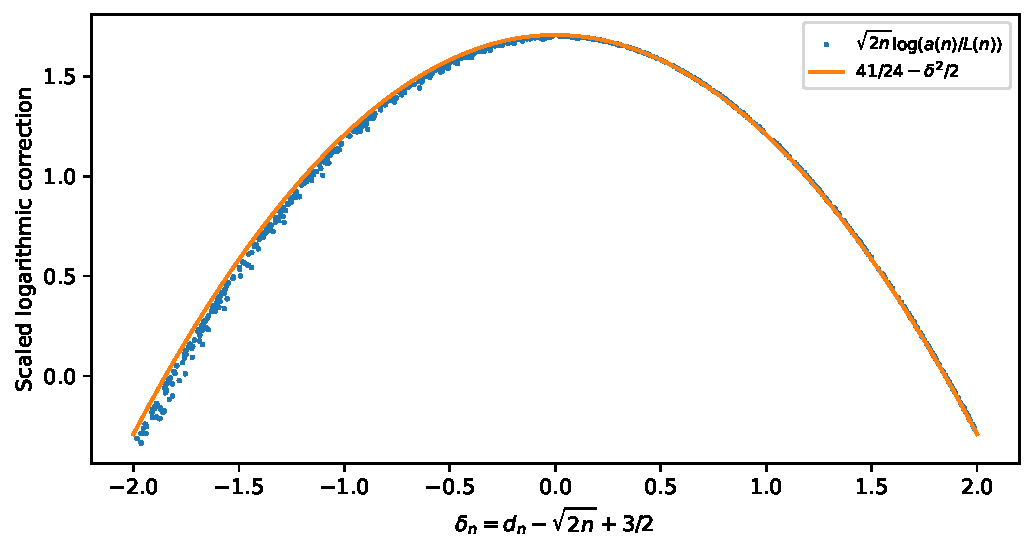
\includegraphics[width=0.93\linewidth]{figures/lattice_correction.pdf}
 \caption{The scaled logarithmic correction versus the exact displacement
 $\delta_n$, sampled for $1000\le n\le16000$. The limiting curve is the
 parabola $P_1(\delta)=41/24-\delta^2/2$. All plotted data are newly computed
 from the formulas in this note.}
 \label{fig:phase}
\end{figure}
\FloatBarrier

\section{Consecutive ratios and their oscillations}\label{sec:ratios}

The OEIS entry links to a plot of $a(n+1)/(a(n)\sqrt n)$
\cite{oeis280}. Its limiting value and its visible fluctuations can both be
settled exactly.

\begin{proposition}[Exact one-step transition]\label{prop:transition}
Write $d=d_n$ and $m=(n-d)/2$. Then
\begin{equation}\label{eq:dtransition}
 d_{n+1}=
 \begin{cases}
 d+1,&d(d+1)<2n+7,\\
 d-3,&d(d+1)>2n+7.
 \end{cases}
\end{equation}
There is no equality case. Correspondingly,
\begin{equation}\label{eq:atransition}
 \frac{a(n+1)}{a(n)}=
 \begin{cases}
 \dfrac{2(n+1)}{d+1},&d_{n+1}=d+1,\\[8pt]
 \dfrac{(n+1)d(d-1)(d-2)}{8(m+1)(m+2)},&d_{n+1}=d-3.
 \end{cases}
\end{equation}
\end{proposition}

\begin{proof}
As $n$ increases by $1$, the integer
$\lfloor\sqrt{8n+21}\rfloor$ increases by either $0$ or $1$. Indeed the
underlying square root increases by less than $1$ even at $n=0$.
Thus \eqref{eq:kexact} shows $k_{n+1}-k_n\in\{0,1\}$, and the only possible
exponents are $d+1$ and $d-3$.

When both candidates exist, compare them using
\eqref{eq:quadraticcriterion}, now at index $n+1$ and lower degree $d-3$.
The deciding expression is
\[
 (d-3)^2+7(d-3)+7-2(n+1)=d^2+d-7-2n.
\]
Its sign gives \eqref{eq:dtransition}. If $d<3$, only the first candidate is
valid, and its displayed inequality automatically holds. Equality is
impossible because $d(d+1)$ is even and $2n+7$ is odd. Finally, cancel
factorials in \eqref{eq:aexact} in each of the two cases to obtain
\eqref{eq:atransition}.
\end{proof}

\begin{theorem}[Ratio limit and sharp fluctuations]\label{thm:ratios}
For $n\ge1$, let
\[
 R_n=\frac{a(n+1)}{a(n)\sqrt n}.
\]
Then
\begin{equation}\label{eq:Rlimit}
 \boxed{\displaystyle R_n\longrightarrow\sqrt2.}
\end{equation}
More precisely, define the continuous, period-$4$ function whose values on
$[-2,2]$ are
\begin{equation}\label{eq:H}
 H(z)=
 \begin{cases}
 \tfrac12-z,&-2\le z\le1,\\
 3z-\tfrac72,&1\le z\le2.
 \end{cases}
\end{equation}
Then
\begin{equation}\label{eq:Rexp}
 \sqrt n\,(R_n-\sqrt2)=H(\delta_n)+O(n^{-1/2}).
\end{equation}
In particular,
\begin{equation}\label{eq:Rsharp}
 \liminf\sqrt n\,(R_n-\sqrt2)=-\frac12,
 \qquad
 \limsup\sqrt n\,(R_n-\sqrt2)=\frac52.
\end{equation}
The empirical distribution of the scaled deviations tends to
$\Unif[-1/2,5/2]$.
\end{theorem}

\begin{proof}
Substitute $d=s-3/2+\delta_n$, $m=(n-d)/2$, and $s=\sqrt{2n}$ into
\eqref{eq:atransition}. In the first case, expansion of the rational
expression gives
\[
 R_n=\sqrt2\left(1+\frac{1/2-\delta_n}{s}+O(s^{-2})\right).
\]
In the second case, the same calculation gives
\[
 R_n=\sqrt2\left(1+\frac{3\delta_n-7/2}{s}+O(s^{-2})\right).
\]
The first branch condition is $\delta_n\le1+O(s^{-1})$, and the second is
$\delta_n\ge1+O(s^{-1})$. Both linear expressions agree at $\delta=1$.
They also agree at the identified endpoints $-2$ and $2$. Consequently the
periodic formula \eqref{eq:Rexp} is uniform even near the switching points
and at the endpoints in \eqref{eq:deltabound}.

The limit and the extreme values follow immediately. For the distribution,
apply Theorem~\ref{thm:deltauniform}. On the first branch, uniform measure
of density $1/4$ is mapped with slope of magnitude $1$; on the second,
with slope $3$. Every interior point of $[-1/2,5/2]$ therefore has total
image density $1/4+1/12=1/3$, which is the uniform density on that interval.
\end{proof}

\begin{figure}[htbp]
 \centering
 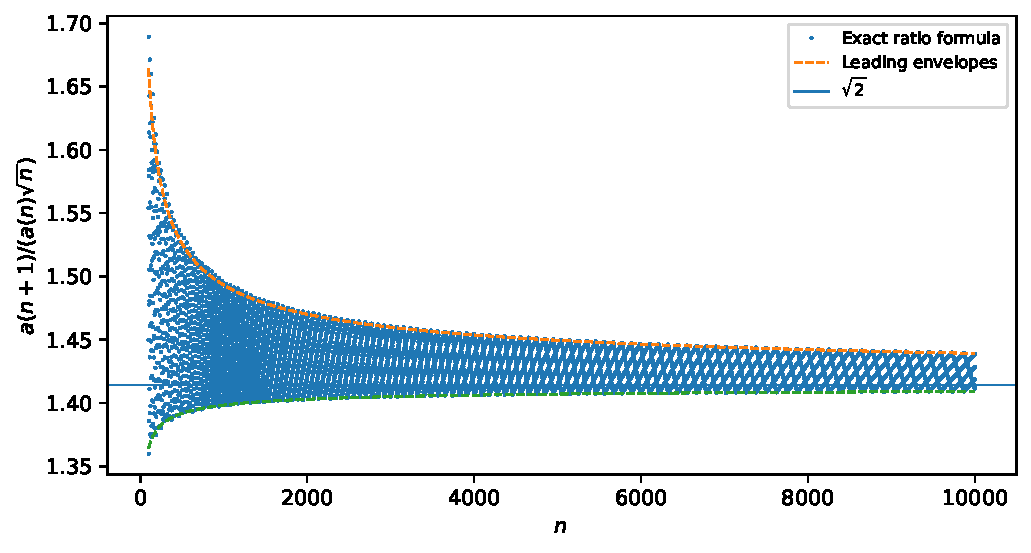
\includegraphics[width=0.93\linewidth]{figures/ratio_convergence.pdf}
 \caption{The ratio $R_n$ for $100\le n\le10000$, computed from the exact
 transition formula. The horizontal line is $\sqrt2$. The other curves,
 $\sqrt2-1/(2\sqrt n)$ and $\sqrt2+5/(2\sqrt n)$, are leading asymptotic
 envelopes, not asserted finite-$n$ inequalities.}
 \label{fig:ratio}
\end{figure}
\FloatBarrier

\section{Comparison with the maximum absolute coefficient}\label{sec:absolute}

Let $b(n)$ denote A277281, the maximum coefficient magnitude
\cite{oeis281}. Its candidate degrees satisfy only $d\equiv n\pmod2$.
For consecutive candidates,
\begin{equation}\label{eq:tworatio}
 \frac{C_n(d+2)}{C_n(d)}
 =\frac{2(n-d)}{(d+1)(d+2)}.
\end{equation}
The threshold is now the root of $d^2+5d+2-2n=0$, namely
\[
 \rho_n=\frac{\sqrt{8n+17}-5}{2}.
\]
Any maximizing exponent $t_n$ lies in $[\rho_n,\rho_n+2]$, with the obvious
restriction to the finite allowed lattice. Ties can occur in this unsigned
problem. For sufficiently large $n$,
\[
 t_n=s_n-\frac32+\varepsilon_n,\qquad
 |\varepsilon_n|\le1+O(s_n^{-1}).
\]
The same Stirling argument therefore gives
\begin{equation}\label{eq:unsigned}
 b(n)\sim L(n),\qquad
 \frac{a(n)}{b(n)}\longrightarrow1.
\end{equation}
More precisely, applying the uniform local expansion to both exponents,
\begin{equation}\label{eq:signedunsigned}
 \log\frac{a(n)}{b(n)}
 =\frac{\varepsilon_n^2-\delta_n^2}{2s_n}+O(s_n^{-2}).
\end{equation}
Thus the sign restriction has a real, rounding-dependent effect at relative
order $n^{-1/2}$, but it does not change the leading constant. As a simple
example of an unsigned tie, $H_8$ has coefficients $13440$ and $-13440$
at degrees $4$ and $2$, respectively. The signed maximum still has the
unique positive maximizing exponent from Theorem~\ref{thm:exact}.

\section{Algorithms, numerical checks, and reproducibility}\label{sec:computation}

\subsection{A single exact term}

The essential implementation is short:
\begin{lstlisting}
from math import factorial, isqrt

def a277280(n: int) -> int:
    if isinstance(n, bool) or not isinstance(n, int):
        raise TypeError("n must be an integer")
    if n < 0:
        raise ValueError("n must be nonnegative")
    k = (2 * n + 6 - isqrt(8 * n + 21)) // 8
    d = n - 4 * k
    return (factorial(n) << d) // (factorial(2 * k) * factorial(d))
\end{lstlisting}
The integer square root is important: the decision is exact even when a
floating-point approximation is too close to a floor boundary to be safe.
The fuller implementation in \texttt{code/a277280.py} also accepts objects
implementing Python's integer-index protocol and exposes the mode separately.

Finding the mode uses one integer square root and a bounded number of
integer arithmetic operations on $O(\log n)$-bit inputs. This is a count
of operations, not a constant-time bit-complexity claim. Evaluating the
coefficient still involves large-integer factorials, products, and a division.
By \eqref{eq:fulllog}, the output itself has $\Theta(n\log n)$ bits, so its
construction and output cannot be constant-time in a bit model.

\subsection{Streaming a prefix}

Proposition~\ref{prop:transition} gives a prefix algorithm that does not
recompute factorials and does not construct Hermite polynomials. Maintain
$(n,d,m,A)$ with $d=d_n$, $m=(n-d)/2$, and $A=a(n)$, initially
$(0,0,0,1)$. If $d(d+1)<2n+7$, replace
\[
 A\leftarrow\frac{2(n+1)A}{d+1},\qquad d\leftarrow d+1,
\]
leaving $m$ unchanged. Otherwise replace
\[
 A\leftarrow\frac{(n+1)d(d-1)(d-2)A}{8(m+1)(m+2)},\qquad
 d\leftarrow d-3,\qquad m\leftarrow m+2.
\]
Then increment $n$. All divisions are exact. The implementation checks the
remainder with \texttt{divmod}, so an implementation error cannot silently
turn into a truncated integer value.

The algorithm uses $O(N)$ transitions for terms through $N$, each involving
a bounded number of operations on the current large integer and factors
of $O(\log N)$ bits. The total binary size of all outputs is
$\Theta(N^2\log N)$, which is a more informative scale than a bare arithmetic
operation count when writing a long b-file.

\subsection{Numerical evaluation without enormous factorials}

For large $n$, compute
\begin{equation}\label{eq:logcompute}
 \log a(n)=\log\Gamma(n+1)-\log\Gamma(m+1)-\log\Gamma(d+1)+d\log2.
\end{equation}
Subtract $\log L(n)$ at high precision, then apply \texttt{exp} or
\texttt{expm1}. In particular, \texttt{expm1} avoids loss of relative
accuracy when evaluating a correction close to zero. Guard precision is
needed because the individual gamma logarithms have size $O(n\log n)$
while their residual after normalization can have size $O(n^{-1/2})$.
The supplied routine adds guard digits based on the size of $n$.

Table~\ref{tab:numeric} compares the leading approximation and its first
two logarithmic corrections. The values were computed at high precision;
the displayed decimals are rounded. The low index $n=10$ is deliberately
included to show that small-$n$ accuracy need not improve monotonically
with the addition of asymptotic terms.

\begin{table}[htbp]
 \centering\small
 \setlength{\tabcolsep}{4.5pt}
 \begin{tabular}{rrccc}
 \toprule
 $n$ & $d_n$ & $a(n)/L(n)$ & $a(n)/L_1(n)-1$ & $a(n)/L_2(n)-1$\\
 \midrule
 $10$ & 2 & $0.9900563798$ & $-2.490\times 10^{-1}$ & $-9.401\times 10^{-2}$ \\
$100$ & 12 & $1.0959224302$ & $-1.452\times 10^{-2}$ & $-2.300\times 10^{-3}$ \\
$1000$ & 44 & $1.0320386856$ & $1.151\times 10^{-4}$ & $-8.533\times 10^{-6}$ \\
$10000$ & 140 & $1.0120994106$ & $-3.108\times 10^{-5}$ & $-9.717\times 10^{-7}$ \\
$10^{6}$ & 1,412 & $1.0010271211$ & $-1.361\times 10^{-6}$ & $-2.373\times 10^{-9}$ \\
$10^{8}$ & 14,140 & $1.0001065067$ & $-1.221\times 10^{-8}$ & $-2.194\times 10^{-12}$ \\
$10^{12}$ & 1,414,212 & $1.0000012066$ & $-4.380\times 10^{-13}$ & $-1.159\times 10^{-18}$ \\
\bottomrule

 \end{tabular}
 \caption{High-precision comparisons using the exact maximizing degree.
 $L_j$ is defined by \eqref{eq:Lj}. More digits and the $L_3$ results appear
 in \texttt{data/asymptotic\_comparison.csv}.}
 \label{tab:numeric}
\end{table}

\begin{figure}[htbp]
 \centering
 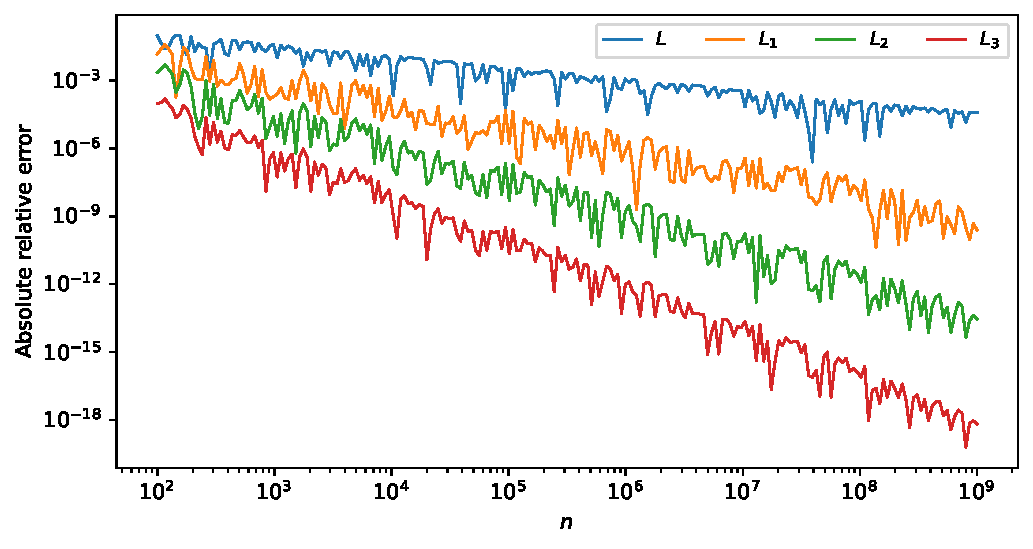
\includegraphics[width=0.93\linewidth]{figures/approximation_errors.pdf}
 \caption{Absolute relative errors of $L,L_1,L_2,L_3$ at logarithmically
 spaced indices. Their proved uniform orders are, respectively,
 $n^{-1/2},n^{-1},n^{-3/2},n^{-2}$. The varying correction polynomials cause
 the fluctuations and occasional near-cancellations.}
 \label{fig:errors}
\end{figure}
\FloatBarrier

\subsection{What was actually checked}

The included verification script completed the following independent checks.
It matched the 25 terms $n=0,\ldots,24$ displayed in the OEIS text entry;
constructed $H_n$ independently from
$H_{n+1}=2xH_n-2nH_{n-1}$ for $n\le300$ and compared its maximum;
and enumerated every positive coefficient for $n\le800$ using exact
coefficient ratios. It also compared the streaming algorithm and the
factorial formula for $n\le1000$.

Further integer checks verified the neighboring-mode inequalities for every
$n\le100000$ and for 500 reproducibly sampled integers below $10^{100}$,
and verified the quartic factorization over all legal adjacent positive
pairs for $n<1000$. High-precision evaluations at eight selected indices
through $10^{12}$ agreed with the analytic Stirling bounds. An additional
SymPy calculation verified all three correction polynomials exactly as
symbolic expressions.

These finite checks support the implementations and algebra, not the
infinite asymptotic conclusions: those follow from the proofs above.
The full external OEIS b-file was not included in the executed comparison;
the script has an optional \texttt{--oeis-file} argument to check it. The
bundled table through $n=1000$ was generated independently by the streaming
algorithm and is explicitly labeled as computed data, not as a downloaded
OEIS reference file.

\subsection{Archive contents and regeneration}

The archive contains \texttt{article.tex} and its compiled PDF; the exact
and high-precision library \texttt{code/a277280.py}; the independent test
script \texttt{code/verify.py}; the table and figure generator
\texttt{code/reproduce.py}; and the optional symbolic calculation
\texttt{code/symbolic\_check.py}. The \texttt{data} directory contains
verification results, a computed b-file through $1000$, and high-precision
comparison data. The \texttt{figures} directory contains the three plots in
both PDF and PNG formats.

The exact algorithms use only the Python standard library. Reproducing
the numerical figures requires \texttt{mpmath}, \texttt{numpy}, and
\texttt{matplotlib}; the optional algebra check uses \texttt{sympy}.
The README and Makefile give the complete regeneration commands. No network
access is needed to rebuild the article or run the supplied checks.

\section{Conclusion}

The asymptotic growth of A277280 is fully determined by
\[
 a(n)\sim\frac{\ee^{-1/2}}{\sqrt\pi\,(2n)^{1/4}}
         \left(\frac{2n}{\ee}\right)^{n/2}\ee^{\sqrt{2n}}.
\]
The key exact fact is that the maximizing positive degree is found by a
single integer square root. Its location is $\sqrt{2n}-3/2$ up to a bounded
lattice-rounding displacement. Stirling's formula then determines not only
the dominant growth, but also the leading constant and a complete scheme
for further corrections.

The rounding displacement matters first at relative order $n^{-1/2}$.
It explains why a smooth constant second term is unavailable, why the
maximum absolute coefficient has the same leading asymptotic, and why the
normalized consecutive ratios oscillate while converging to $\sqrt2$.
All statements hold along the full sequence, without an unmentioned parity
subsequence or averaging assumption.

\begin{thebibliography}{9}
\bibitem{oeis280}
Vladimir Reshetnikov and OEIS contributors,
\emph{A277280: Maximal coefficient in Hermite polynomial of order n},
The On-Line Encyclopedia of Integer Sequences.
Created 8 October 2016; text entry consulted 20 September 2026.
\url{https://oeis.org/A277280}.
The entry credits Vaclav Kotesovec for a numerical table and a ratio plot.

\bibitem{dlmfhermite}
National Institute of Standards and Technology,
\emph{Digital Library of Mathematical Functions},
Section 18.5, equation 18.5.13: explicit finite expansion of $H_n$.
\url{https://dlmf.nist.gov/18.5.E13}.
Consulted 20 September 2026.

\bibitem{dlmfgamma}
National Institute of Standards and Technology,
\emph{Digital Library of Mathematical Functions},
Section 5.11: asymptotic expansions of the gamma function;
in particular equation 5.11.1 and Section 5.11(ii), remainder bounds.
\url{https://dlmf.nist.gov/5.11}.
Consulted 20 September 2026.

\bibitem{oeis281}
Vladimir Reshetnikov and OEIS contributors,
\emph{A277281: Maximal absolute value of coefficients in Hermite polynomial
of order n}, The On-Line Encyclopedia of Integer Sequences.
\url{https://oeis.org/A277281}.
Consulted 20 September 2026.
\end{thebibliography}
\end{document}
